% === Fig. 1: OpenCLIP raw-v2 CPU runtime smoke test ===
\begin{figure}[t]
\centering
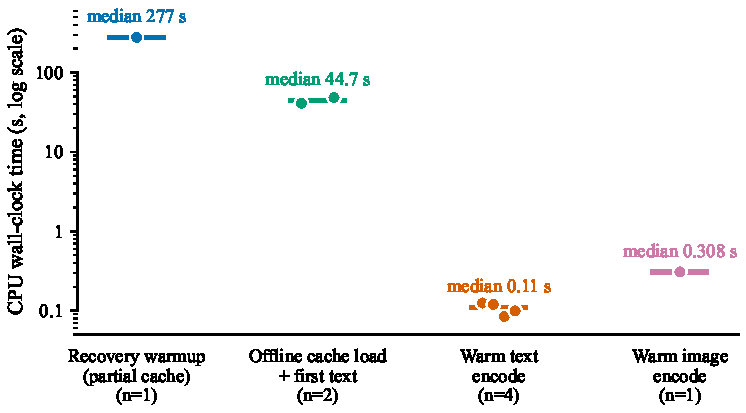
\includegraphics[width=0.95\columnwidth]{figures/fig1_openclip_raw_v2_runtime.pdf}
\caption{CPU wall-clock observations for distinct OpenCLIP raw-v2 execution regimes on an Intel Core Ultra 7 255HX. Points are raw observations and horizontal ticks are medians; no confidence intervals are estimated because each regime has only $n=1$--$4$. The 276.544-s recovery warmup completed a prior partial cache and includes download, validation, model load, and warmup, so it is not a clean cold-download measurement. Offline cached-load trials use fresh Python processes. The smoke test verified finite, unit-normalized 512-D vectors and preserved raw Unicode Chinese input; it does not measure retrieval accuracy.}
\label{fig:openclip-runtime}
\end{figure}

\begin{table}[t]
\centering
\caption{Embedding-provider capability taxonomy. This table describes implementation roles, not retrieval quality.}
\label{tab:embedding-provider-taxonomy}
\begin{tabular}{lcccl}
\toprule
Provider & Dim. & Joint image--text model & Language path & Project role \\
\midrule
Lightweight semantic v1 & 16 & No & Bounded dictionary & Handcrafted baseline \\
OpenCLIP raw v2 & 512 & Yes & Raw multilingual XLM-R & Learned default; runtime measured \\
OpenCLIP bridge v1 & 512 & Yes & Chinese keyword bridge & Legacy ablation \\
\bottomrule
\end{tabular}
\end{table}


% === Fig. 2: Production-equivalent multilingual retrieval proxy pilot ===
\begin{figure*}[t]
\centering
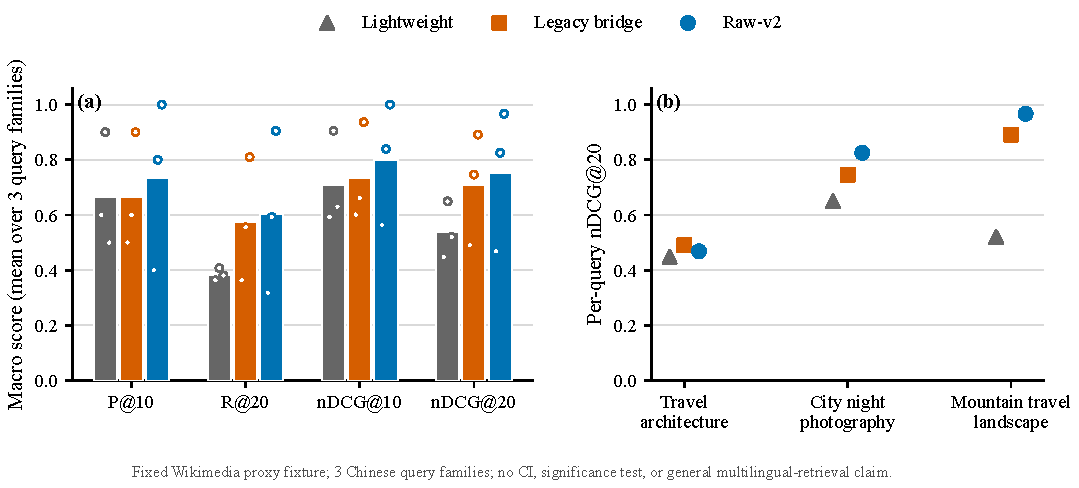
\includegraphics[width=0.95\textwidth]{figures/fig2_openclip_raw_v2_proxy_retrieval.pdf}
\caption{Retrieval comparison on a fixed 81-candidate proxy fixture using three Chinese query families. Panel (a) reports macro means as bars and overlays the three query-family observations as open circles; panel (b) exposes per-family nDCG@20 so the aggregate does not hide the weaker raw-v2 architecture result. The legacy bridge reuses raw-v2 image vectors and changes only Chinese text preparation. Rankings follow the production contract: cosine scores rounded to six decimals, then quality score and stable photo UUID. The 72 labels are inherited from Wikimedia download search terms rather than blind human judgments, and nine unjudged synthetic derivatives count as non-relevant. With only three query families, no confidence interval, statistical-significance conclusion, or general multilingual-retrieval claim is reported.}
\label{fig:openclip-raw-v2-proxy}
\end{figure*}

\begin{table*}[t]
\centering
\caption{Macro retrieval results under one production-equivalent ranking run. Each row averages the same three query families over 81 candidates (72 Wikimedia search-term proxy labels; nine unjudged synthetic derivatives count as non-relevant). These deterministic pilot values have no confidence intervals and support no significance claim. Legacy bridge reuses the raw-v2 image vectors and changes only the Chinese text preparation.}
\label{tab:openclip-raw-v2-proxy}
\small
\setlength{\tabcolsep}{4pt}
\begin{tabular}{llccccc}
\toprule
Language & Provider / query path & MRR & P@10 & R@20 & nDCG@10 & nDCG@20 \\
\midrule
English & Lightweight & 1.000 & 0.667 & 0.384 & 0.709 & 0.539 \\
English & Raw-v2 & 1.000 & 0.800 & 0.608 & 0.822 & 0.746 \\
\midrule
Chinese & Lightweight & 1.000 & 0.667 & 0.384 & 0.709 & 0.539 \\
Chinese & Legacy bridge & 1.000 & 0.667 & 0.576 & 0.733 & 0.710 \\
Chinese & Raw-v2 & 1.000 & 0.733 & 0.605 & 0.801 & 0.753 \\
\bottomrule
\end{tabular}
\end{table*}


% === Fig. S1: Windows NumPy/Torch native-runtime compatibility ===
\begin{figure*}[t]
\centering
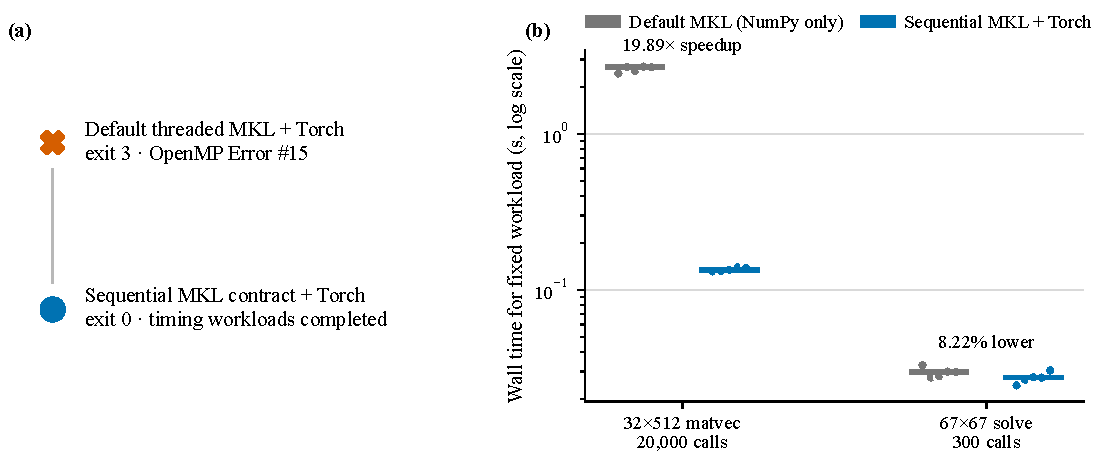
\includegraphics[width=0.95\textwidth]{figures/figS1_windows_numeric_runtime.pdf}
\caption{Windows native-runtime compatibility and representative small-matrix timing. Panel (a) records one reproduction of OpenMP Error \#15 before the runtime contract and a successful process after selecting sequential MKL; the unsafe \texttt{KMP\_DUPLICATE\_LIB\_OK} workaround was not used. Panel (b) shows all five wall-clock observations and median ticks for two fixed NumPy workloads. Default MKL was measured without Torch because the mixed default process aborts; the safe condition includes Torch and sequential MKL. This is a single-machine engineering compatibility profile, not a general BLAS or end-to-end model-speed claim.}
\label{fig:windows-numeric-runtime}
\end{figure*}

\begin{table*}[t]
\centering
\caption{Windows numeric-runtime compatibility profile. Times are five-repeat medians for fixed workloads on one machine. The default arm uses NumPy without Torch because default MKL plus Torch aborts; the safe arm uses sequential MKL with Torch loaded.}
\label{tab:windows-numeric-runtime}
\small
\begin{tabular}{lrrr}
\toprule
Workload & Default MKL & Sequential + Torch & Change \\
\midrule
32$\times$512 matvec ($20{,}000$ calls) & 2.678 s & 0.1346 s & 19.89$\times$ speedup \\
67$\times$67 solve ($300$ calls) & 0.02986 s & 0.02741 s & 8.22\% lower \\
\bottomrule
\end{tabular}
\end{table*}


% === Fig. 5: Real learned-model runtime and timing integrity ===
% Generated by gen_fig5_model_backed_runtime_integrity.py
\begin{figure*}[t]
  \centering
  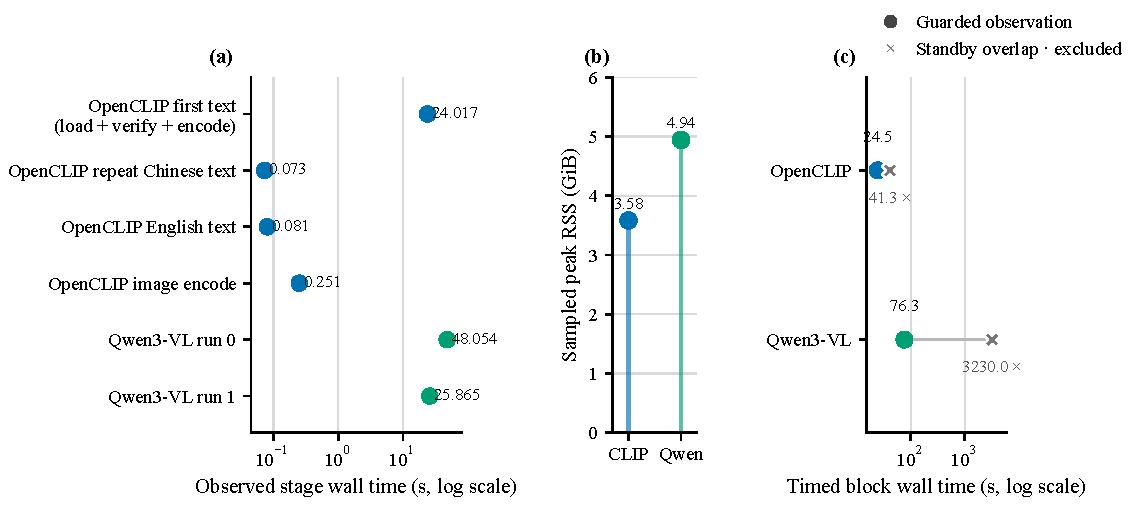
\includegraphics[width=\textwidth]{figures/fig5_model_backed_runtime_integrity.pdf}
  \caption{Real CPU inference observations for the pinned learned OpenCLIP and Qwen3-VL stack. (a) Raw clean stage timings; points are individual observations, not distributions. (b) 50-ms sampled process RSS peaks. (c) Modern-Standby-overlap observations are retained for audit but excluded from latency claims; guarded runs are not interpreted as model speedups. Functional vector/output payloads were unchanged. The smokes do not evaluate retrieval quality or semantic entailment.}
  \label{fig:model-backed-runtime-integrity}
\end{figure*}
\begin{table*}[t]
\centering
\caption{Single-machine learned-model functional smokes on an Intel Core Ultra 7 255HX (20 cores, 32 GB class RAM), Windows 11 build 26200, CPU inference. Values are raw observations without confidence intervals. OpenCLIP first text includes model load, manifest verification, and encode; Qwen run 0 excludes Python/Torch import and the pre-timing weight hash. RSS is sampled every 50 ms.}
\label{tab:model-backed-runtime-integrity}
\small
\setlength{\tabcolsep}{4pt}
\begin{tabular}{llrrl}
\toprule
Model & Observation & Time (s) & Peak RSS (GiB) & Scope \\
\midrule
OpenCLIP & First text (load + verify + encode) & 24.017 & 3.582 & $n=1$ functional smoke \\
OpenCLIP & Repeat Chinese text / image encode & 0.073 / 0.251 & -- & same process \\
Qwen3-VL & Grounded generation run 0 & 48.054 & 4.944 & referential validation only \\
Qwen3-VL & Grounded generation run 1 & 25.865 & -- & same canonical output \\
\bottomrule
\end{tabular}
\end{table*}



% === Fig. 6: Mutable public-fixture reconstruction audit ===
% Generated by gen_fig6_wikimedia_fixture_drift.py
\begin{figure*}[t]
  \centering
  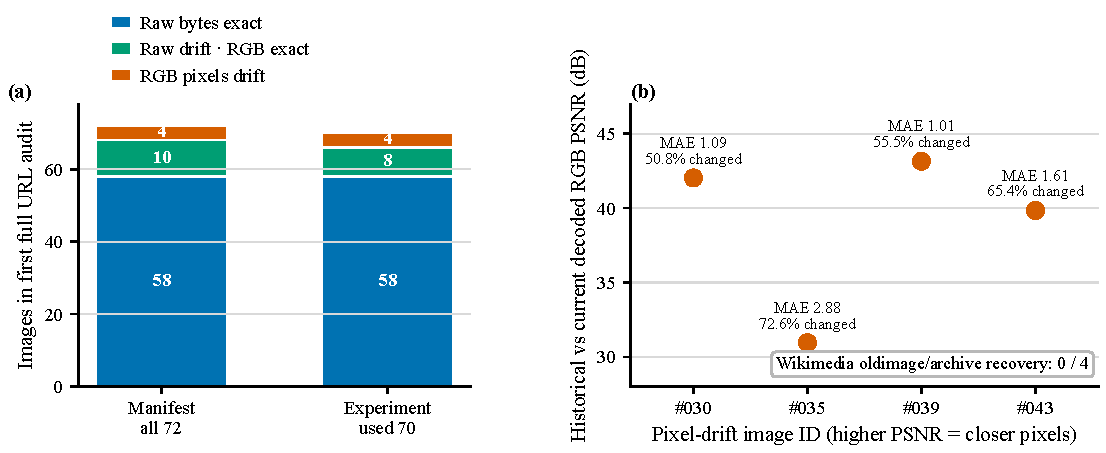
\includegraphics[width=\textwidth]{figures/fig6_wikimedia_fixture_drift.pdf}
  \caption{Mutable-upstream audit of the historical 72-image Wikimedia fixture. (a) Only 58 responses remained byte-identical; ten changed only JPEG metadata while preserving decoded RGB, and four changed decoded pixels. (b) The four pixel-drift cases differ measurably despite unchanged dimensions. No historical raw or pixel-drift input was recovered through Wikimedia oldimage/archive. The existing experiment keeps its historical raw-SHA provenance and the downloader fails closed; exact fresh-clone replay requires a separately licensed content-addressed archive or a new experiment ID. The public artifact freezes historical pins and the audit summary, not transient current-response binaries or the complete per-file archive transcript; current-side differences are contemporaneous audit-record observations rather than independently offline-replayable measurements.}
  \label{fig:wikimedia-fixture-drift}
\end{figure*}
\begin{table*}[t]
\centering
\caption{Reconstruction audit for the mutable Wikimedia thumbnail URLs used by the historical preference-study fixture. Percentages describe one sequential full pass on 2026-08-29; they are not availability guarantees.}
\label{tab:wikimedia-fixture-drift}
\small
\begin{tabular}{lrrrr}
\toprule
Scope & Raw exact & Raw drift / RGB exact & RGB drift & Archive recovery \\
\midrule
All manifest images ($n=72$) & 58 (80.56\%) & 10 (13.89\%) & 4 (5.56\%) & raw 0 / 14; pixels 0 / 4 \\
Experiment-used images ($n=70$) & 58 (82.86\%) & 8 (11.43\%) & 4 (5.71\%) & raw 0 / 12; pixels 0 / 4 \\
\bottomrule
\end{tabular}
\end{table*}


